\chapter{String Theory and M-Theory}

Susskind begins this lecture in the way he says he has come to like: not by attacking the main problem head on, but by clearing the ground with two preliminaries. First comes a rapid harmonic-oscillator review, done not because the audience has never seen it, but because the notation for string modes must be fixed before anything else can be interpreted. Then comes a review of the spin of massless particles. Only after those two pieces are in place does the lecture turn to the low-lying spectrum of the string. We keep that order here. The transcript is the primary guide, while the preserved blackboard frames serve as local evidence for equations and board layout. In that spirit these notes explicitly preserve the lecture of Leonard Susskind and the supporting curation work of LazyingArt LLC and Video2Book.

\section{Rapid Harmonic-Oscillator Review for String Modes}

We begin exactly where the lecture begins: with the warning that this is only a quick reset of notation. The \(n\)th mode of the open string behaves like a harmonic oscillator, and the index \(n\) is the same \(n\) that appears in the mode function \(\cos n\sigma\). It counts how many oscillations fit along the interval \(0\leq \sigma\leq \pi\). The only unusual feature is a normalization inherited from the string calculation: a factor of \(4\) appears in the denominator, and Susskind is quite explicit that we should simply keep it.

\begin{figure}[t]
\centering

\includegraphics[width=0.62\textwidth]{lecture_03_figure_02.png}
\caption{Harmonic oscillator energy and Lagrangian.}
\end{figure}

The first blackboard frame is useful not because it reveals every symbol perfectly, but because it preserves the comparison the lecture is making. The upper and lower lines contain the same quadratic pieces, and only the sign of the potential term changes. The right-hand labels are cropped, so we stabilize them from the transcript:
\begin{align}
E_n &= \frac{\dot X_n^{\,2}}{4}+\frac{n^2X_n^{\,2}}{4}, \\
L_n &= \frac{\dot X_n^{\,2}}{4}-\frac{n^2X_n^{\,2}}{4}.
\end{align}
The point is simple: the \(n\)th mode is an oscillator of frequency \(n\). That is what we want to carry forward.

Now we do the first standard step toward quantization. At the board Susskind suppresses the label \(n\) for a moment and writes the single oscillator coordinate simply as \(x\). From the Lagrangian,
\begin{equation}
p=\frac{\partial L}{\partial \dot x}=\frac{\dot x}{2},
\end{equation}
so \(\dot x=2p\). Substituting back into the energy gives the Hamiltonian
\begin{equation}
H=p^2+\frac{n^2x^2}{4}.
\end{equation}
So far nothing mysterious has happened. We have merely rewritten the same oscillator in Hamiltonian form.

\section{Hamiltonian, Ladder Operators, and the Return to the String}

The next move is the usual oscillator trick, and Susskind presents it in the usual brisk, heuristic way. Since
\begin{equation}
H=p^2+\left(\frac{nx}{2}\right)^2,
\end{equation}
we are naturally led to the complex combinations
\begin{equation}
\frac{nx}{2}\pm ip.
\end{equation}
At the blackboard this is phrased as a factorization of the sum of squares,
\begin{equation}
H \sim \left(\frac{nx}{2}+ip\right)\left(\frac{nx}{2}-ip\right),
\end{equation}
and the point is not a polished discussion of operator ordering. The point is that these are the combinations out of which the creation and annihilation operators are built.

To normalize them we must check the commutator. With \(\hbar=1\),
\begin{equation}
[x,p]=i.
\end{equation}
Let us check what the tentative pair does:
\begin{align}
\left[\frac{nx}{2}+ip,\frac{nx}{2}-ip\right]
&=
-\frac{ni}{2}[x,p]+\frac{ni}{2}[p,x] \\
&=
-\frac{ni}{2}(i)+\frac{ni}{2}(-i) \\
&= \frac{n}{2}+\frac{n}{2}=n.
\end{align}
So the natural combinations almost work, but not quite. Their commutator is \(n\), not \(1\). The fix is immediate: divide by \(\sqrt n\). Thus
\begin{align}
a^- &= \frac{1}{\sqrt n}\left(\frac{nx}{2}+ip\right)
= \frac{\sqrt n\,x}{2}+\frac{i}{\sqrt n}p, \\
a^+ &= \frac{1}{\sqrt n}\left(\frac{nx}{2}-ip\right)
= \frac{\sqrt n\,x}{2}-\frac{i}{\sqrt n}p,
\end{align}
and now
\begin{equation}
[a^-,a^+]=1.
\end{equation}
The lecture makes an instructive point here. One cannot read off from the visible minus sign alone which operator raises the energy and which lowers it. The criterion is the commutator. The convention above is the one for which \(a^+\) is the raising operator and \(a^-\) is the lowering operator.

Once the string is taken to move with very large momentum along the \(z\)-axis, the independent oscillations are transverse. In three space dimensions there are therefore two copies of the oscillator, one in the \(x\)-direction and one in the \(y\)-direction. We introduce a second pair,
\begin{align}
b^- &= \frac{\sqrt n\,y}{2}+\frac{i}{\sqrt n}p_y, \\
b^+ &= \frac{\sqrt n\,y}{2}-\frac{i}{\sqrt n}p_y,
\end{align}
with
\begin{equation}
[b^-,b^+]=1.
\end{equation}

\begin{figure}[t]
\centering

\includegraphics[width=0.62\textwidth]{lecture_03_figure_03.png}
\caption{Commutators for the \(a\)- and \(b\)-oscillator modes.}
\end{figure}

The second blackboard frame is especially valuable because it shows the lecture's organization: first the commutator block, then a dividing line, and only then the explicit operator formulas. In cleaned form the upper block is
\begin{equation}
[a^-,a^+]=1,\qquad [b^-,b^+]=1,\qquad [x,p]=i.
\end{equation}
The lower part of the frame only begins the formula for \(a^-\), so the full coefficients are stabilized from the transcript.

Now comes the step that turns the oscillator algebra back into the string. Adding the two defining equations for \(a_n^\pm\) eliminates the momentum term and gives
\begin{equation}
a_n^++a_n^-=\sqrt n\,x_n.
\end{equation}
Hence
\begin{equation}
x_n=\frac{a_n^++a_n^-}{\sqrt n},\qquad
y_n=\frac{b_n^++b_n^-}{\sqrt n}.
\end{equation}
This is not bookkeeping for its own sake. It is the bridge back from the abstract oscillator to the string coordinate itself.

The open string is parameterized by \(\sigma\in[0,\pi]\). Its transverse coordinates are expanded in cosine modes,
\begin{align}
x(\sigma,\tau) &= \sum_n x_n(\tau)\cos n\sigma, \\
y(\sigma,\tau) &= \sum_n y_n(\tau)\cos n\sigma.
\end{align}
Why cosines and not sines? Because the endpoint condition is
\begin{equation}
\partial_\sigma x\big|_{\sigma=0,\pi}=0,\qquad
\partial_\sigma y\big|_{\sigma=0,\pi}=0,
\end{equation}
so the slope vanishes at the endpoints. Substituting the operator expressions for the Fourier coefficients yields
\begin{align}
x(\sigma,\tau) &= \sum_n \frac{a_n^++a_n^-}{\sqrt n}\cos n\sigma, \\
y(\sigma,\tau) &= \sum_n \frac{b_n^++b_n^-}{\sqrt n}\cos n\sigma.
\end{align}
This is why the lecture spent time on the oscillator review. Once the coordinate operators are written in terms of creation and annihilation operators, the action of those coordinates on a quantum state becomes transparent.

\begin{figure}[t]
\centering
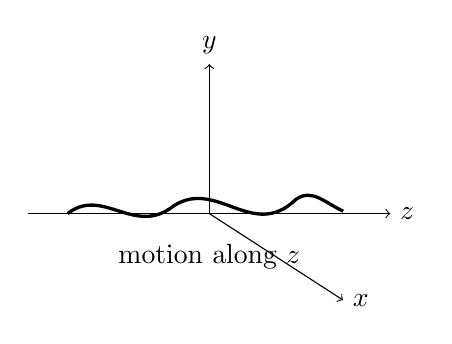
\begin{tikzpicture}[scale=1.0]
\draw[->] (-2.3,0)--(2.3,0) node[right] {$z$};
\draw[->] (0,0)--(0,1.9) node[above] {$y$};
\draw[->] (0,0)--(1.7,-1.1) node[right] {$x$};
\draw[very thick] (-1.8,0) .. controls (-1.35,0.35) and (-0.95,-0.30) .. (-0.45,0.10)
                  .. controls (0.10,0.45) and (0.55,-0.35) .. (1.10,0.18)
                  .. controls (1.30,0.32) and (1.45,0.15) .. (1.70,0.03);
\draw (0,-0.55) node {motion along \(z\)};
\end{tikzpicture}
\caption{The string is taken to move with large momentum along the \(z\)-axis. The independent oscillations are transverse, in the \(x\)- and \(y\)-directions.}
\end{figure}

\subsection{Question \& Answer}

\paragraph{Question.} Do the coefficients \(x_n\) depend on \(\sigma\)?

\paragraph{Answer.} No. All of the \(\sigma\)-dependence is carried by the cosine functions. The coefficients \(x_n\) and \(y_n\) are Fourier coefficients. In the present discussion they depend on the time variable \(\tau\), because the modes themselves oscillate in time. The dots in the oscillator formulas are therefore \(\tau\)-derivatives, not derivatives with respect to the spatial parameter \(\sigma\).

\section{Massive Versus Massless Spin}

With the notation now under control, the lecture turns to the second preliminary. The question is not merely how many states a spin-\(J\) system has, but why the answer changes when the particle is massless.

For a massive particle,
\begin{equation}
N_{\mathrm{massive}}(J)=2J+1.
\end{equation}
Thus spin \(0\) has one state, spin \(1\) has three, spin \(2\) has five, and so forth. But for massless particles the pattern changes sharply:
\begin{equation}
N_{\mathrm{massless}}(0)=1,\qquad
N_{\mathrm{massless}}(s>0)=2.
\end{equation}
Spin \(1\) no longer has three states; it has two. Spin \(2\) no longer has five states; it also has two. Spin \(0\) remains the special case.

The way Susskind builds this is through motion along a chosen axis, say the \(z\)-axis. A spin-\(1\) particle can have spin component \(+1\), \(0\), or \(-1\) along that axis. A spin-\(2\) particle can have \(+2,+1,0,-1,-2\). Reflection symmetry already guarantees that maximal positive and maximal negative helicity must come together. The real issue is whether the intermediate states are forced on us.

For a massive particle they are forced on us, because we can go to its rest frame. One imagines following the particle until it is at rest. Once it is at rest, rotation invariance tells us that if one spin orientation is allowed, then rotated ones are allowed as well. We can then boost back to a moving frame and obtain states whose spin is no longer simply maximal or minimal along the original direction of motion. That is why the full multiplet must be present for a massive particle.

For a massless particle the argument collapses at the first step. There is no rest frame. One cannot bring the particle to rest, rotate it there, and then boost back. The missing rest frame is exactly what allows the intermediate states to disappear. In the massless case it is consistent to keep only the two helicity states of maximal and minimal spin along the direction of motion.

\subsection{Question \& Answer}

\paragraph{Question.} Why do massless particles have only two polarization states?

\paragraph{Answer.} Because the rotate-then-boost argument requires a rest frame. A massive particle can be brought to rest, and once it is at rest the spin can be reoriented and then boosted back into motion, generating the full \(2J+1\) multiplet. A massless particle cannot be brought to rest, so that construction is unavailable. The theory can therefore consistently retain only the two extreme helicity states.

\section{Photon Polarization as the Model Case}

The lecture now translates the abstract spin discussion into the familiar language of photons. This is not a change of topic. It is the concrete model for what will happen to the first excited open-string states a few minutes later.

A photon moving along the \(z\)-axis is polarized in the transverse \(xy\)-plane. The electric field never points along the direction of motion; Maxwell's equations forbid such a longitudinal polarization. Thus the photon has two transverse basis states, which we may call \(|x\rangle\) and \(|y\rangle\). These are linearly polarized states. From them we build the circular basis,
\begin{equation}
|R\rangle=|x\rangle+i|y\rangle,\qquad
|L\rangle=|x\rangle-i|y\rangle.
\end{equation}
These are not normalized states here; they are the lecture's operational basis vectors, and that is enough for the present purpose.

What matters is that the circular combinations are helicity eigenstates. They are the two genuine spin states of the photon. Linear polarization is different. A state such as \(|x\rangle+|y\rangle\) is still only a superposition of the same two physical states; it is simply linearly polarized at a rotated angle in the transverse plane. The complex unit \(i\) is what converts the linear basis into the circular one.

\begin{figure}[t]
\centering
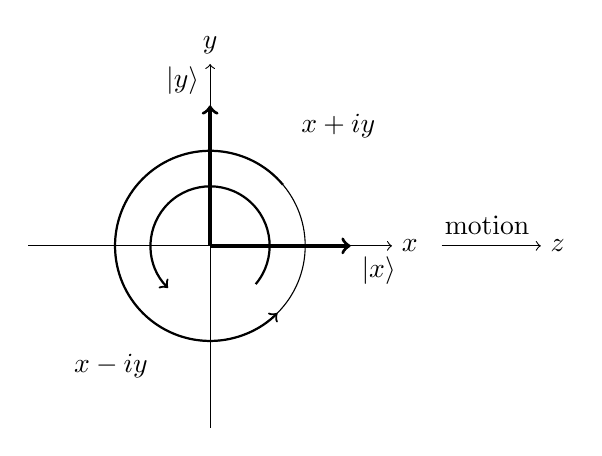
\begin{tikzpicture}[scale=1.05]
\draw[->] (-2.2,0)--(2.2,0) node[right] {$x$};
\draw[->] (0,-2.2)--(0,2.2) node[above] {$y$};
\draw[very thick,->] (0,0)--(1.7,0) node[below right] {$|x\rangle$};
\draw[very thick,->] (0,0)--(0,1.7) node[above left] {$|y\rangle$};
\draw (0,0) circle (1.15);
\draw[thick,->] (40:1.15) arc (40:315:1.15);
\draw[thick,->] (-40:0.72) arc (-40:225:0.72);
\draw (1.55,1.45) node {$x+iy$};
\draw (-1.20,-1.45) node {$x-iy$};
\draw[->] (2.8,0)--(4.0,0) node[right] {$z$};
\draw (3.35,0.25) node {motion};
\end{tikzpicture}
\caption{Linear and circular polarization in the plane transverse to the motion.}
\end{figure}

The same logic also gives the useful graviton analogy. A massless spin-\(2\) particle again has only two states. One may think of them, heuristically, as the analog of two photons of like helicity combined. That way of speaking is useful for spin counting, but the lecture is careful not to turn it into a literal claim that a graviton is made of two photons.

\subsection{Question \& Answer}

\paragraph{Question.} Does linear polarization mean zero angular momentum?

\paragraph{Answer.} Not as a sharp quantum number. A linearly polarized photon is a superposition of the two helicity eigenstates. Its average angular momentum along the direction of motion may vanish, but a measurement never produces a third state of zero helicity. It produces one helicity or the other.

\section{The First Excited Open-String States and the Photon-Like Interpretation}

At this point the lecture cashes in both preliminaries. Susskind explicitly recaps: now we know something about harmonic oscillators, and now we know something about spin. So now we can look at the spectrum.

Before listing states, he reminds us of one essential point of interpretation. In this formal analogy between the string oscillators and relativistic particle states, the oscillator energy contributes to \(m^2\), not directly to \(m\). So when we say that an excitation adds one unit of energy, we mean one unit of mass-squared in the lecture's units.

Let \(|0\rangle\) denote the unexcited string state. This is not empty space. It is a single string whose oscillators are all as quiet as quantum mechanics allows:
\begin{equation}
a_n^-|0\rangle=0,\qquad b_n^-|0\rangle=0
\end{equation}
for every mode \(n\). The lecture deliberately leaves its mass-squared undetermined:
\begin{equation}
m^2(|0\rangle)=m_0^2.
\end{equation}
That unknown is the stage on which the next argument plays out.

What is the cheapest thing we can do to the string? We apply a raising operator to the oscillator of smallest frequency, namely the \(n=1\) mode. This gives two states,
\begin{equation}
a_1^+|0\rangle,\qquad b_1^+|0\rangle.
\end{equation}
Since the \(n\)th oscillator adds \(n\) units, these states have
\begin{equation}
m^2=m_0^2+1.
\end{equation}
The lecture briefly pauses here to note that the actual physical scale hidden in that ``\(1\)'' has not yet been discussed. The units are missing and will be taken up later. But the internal logic does not wait for that discussion.

There is another essential point. The states \(a_1^+|0\rangle\) and \(b_1^+|0\rangle\) are degenerate, so any linear combination of them is again an eigenstate with the same value of \(m^2\). In particular,
\begin{equation}
\left(a_1^+\pm i\,b_1^+\right)|0\rangle
\end{equation}
gives the circularly polarized combinations.

Now the transformation argument arrives. These operators came from the transverse coordinates \(x\) and \(y\). Under rotations about the preferred \(z\)-axis they mix exactly as the components of a two-dimensional vector mix. So the first excited open-string states transform exactly like the two transverse polarization states of a photon. There is no third state of the same energy, because there is no third independent transverse oscillator in this three-dimensional discussion.

That is the crucial payoff. If an object carries only two transverse polarization states, then the only relativistically consistent interpretation is that it is massless. A massive spin-\(1\) particle would have to carry a third polarization state, because it could be brought to rest and rotated. Therefore these states must be massless. The conclusion is
\begin{equation}
m_0^2+1=0.
\end{equation}
So the first excited open-string states are photon-like, or more generally gauge-boson-like, and they are necessarily massless.

The lecture is careful with the language here. It is too fast, and too model-dependent, to say that we have found \emph{the} photon. What we have found is a photon-like object. Historically this mattered. In the old hadronic interpretation of string theory, such a massless spin-\(1\) state was viewed as a wart rather than a feature, because there are no massless mesons. But in the present logical arc it is a success first. Only then does it become a problem.

\section{The Tachyonic Ground-State Disaster}

And now the sharp turn. The first excited state has come out beautifully: it is massless, transverse, and photon-like. But the very condition that makes it so,
\begin{equation}
m_0^2+1=0,
\end{equation}
forces the ground state to have
\begin{equation}
m_0^2=-1
\end{equation}
in the lecture's units. So the success of the first excited state immediately produces the failure of the ground state. This is the moment in the lecture where Susskind says, with deliberate drama, that perhaps we should simply throw the theory away.

\subsection{Question \& Answer}

\paragraph{Question.} Does negative mass-squared mean faster-than-light propagation?

\paragraph{Answer.} Not in the sense relevant to real physics. The name ``tachyon'' arose from a naive reading of the dispersion relation, but the lesson the lecture wants us to keep is different. Negative mass-squared signals an instability of the vacuum. The disease is not useful superluminal signaling; it is that we have expanded the theory around the wrong configuration.

To see how the older language arose, Susskind first recalls the group-velocity rule
\begin{equation}
v_g=\frac{dE}{dp}.
\end{equation}
For a nonrelativistic particle,
\begin{equation}
E(p)=\frac{p^2}{2m},
\qquad
\frac{dE}{dp}=\frac{p}{m},
\end{equation}
which is just the ordinary velocity. For a relativistic particle, in units with \(c=1\),
\begin{equation}
E=\sqrt{p^2+m^2},
\qquad
\frac{dE}{dp}=\frac{p}{\sqrt{p^2+m^2}}.
\end{equation}
As long as \(m^2>0\), this is less than \(1\). If one naively flips the sign of \(m^2\), the algebra suggests a velocity larger than \(1\), and that is why the old term ``tachyon'' stuck.

But now the lecture changes the question. What does negative mass-squared really mean? The answer is not in the kinematics of a single particle, but in the stability of the field configuration. The safe relation to extract from the somewhat sign-corrected wave-equation discussion is
\begin{equation}
\omega^2=k^2+m^2.
\end{equation}
Correspondingly, the quadratic part of the field energy is
\begin{equation}
\mathcal{E}_\phi
=
\frac12\left[(\partial_t\phi)^2+(\partial_x\phi)^2+m^2\phi^2\right].
\end{equation}
If \(m^2>0\), then displacing the field costs positive potential energy, and the system behaves like an ordinary harmonic oscillator. If \(m^2<0\), the quadratic potential near \(\phi=0\) is inverted:
\begin{equation}
V(\phi)\propto -|m|^2\phi^2.
\end{equation}
So \(\phi=0\) is not a minimum at all. It is the top of a hill.

\begin{figure}[t]
\centering
\begin{tikzpicture}[scale=0.95]
\begin{scope}[xshift=-3.6cm]
\draw[->] (-2,0)--(2,0) node[right] {$\phi$};
\draw[->] (0,-0.2)--(0,2.2) node[above] {$V$};
\draw[domain=-1.7:1.7,smooth,variable=\x,thick] plot ({\x},{0.42*\x*\x});
\draw (0,-0.55) node {stable};
\end{scope}
\begin{scope}[xshift=3.6cm]
\draw[->] (-2,0)--(2,0) node[right] {$\phi$};
\draw[->] (0,-2.2)--(0,0.5) node[above] {$V$};
\draw[domain=-1.7:1.7,smooth,variable=\x,thick] plot ({\x},{-0.42*\x*\x});
\draw (0,-2.65) node {tachyonic};
\end{scope}
\end{tikzpicture}
\caption{Positive mass-squared gives an ordinary quadratic potential; negative mass-squared turns the quadratic term upside down and makes \(\phi=0\) unstable.}
\end{figure}

This is why the lecture turns to the pencil, pendulum, and domino analogies. A perfectly balanced pencil can in principle sit forever, but the slightest push sends it away. A row of coupled inverted pendulums behaves similarly: disturb one of them, and an instability front propagates through the system. Yet that front does not outrun the characteristic wave speed. The instability spreads causally. So the right reading of the tachyon is not ``faster than light,'' but ``unstable vacuum.''

The lecture then makes a very pointed comparison. A quantum theory with an upside-down potential is not nonsense in the formal sense. One can write it down. What it lacks is a ground state. That is the real problem. The bosonic open string, taken in this simple form, does not look like the world. It gives us a beautiful photon-like state, but it gives it to us on top of an unstable vacuum. That is why one eventually needs superstring theory.

\section{Rotating Strings, Joining and Splitting, Closed Strings, and Gravity}

Before the final pivot to gravity, the lecture pauses to note that the open-string state we have just identified is not merely a formal polarization count. Once one introduces charged string states and the interaction rules, the emission and absorption patterns match the familiar behavior of gauge bosons. That thread is not pursued mathematically here, because Susskind wants to move to the next indispensable idea: closed strings.

He begins that move by reminding us that the free string can do more than vibrate in simple transverse modes. It can also rotate, and when it rotates it carries angular momentum. In the quantum theory each extra unit of angular momentum costs extra energy. So the string naturally supports towers of higher-spin excitations. This matters because it prepares us to think of string states not just as particles, but as particles with very definite transformation properties.

Now comes the interaction rule, presented quite explicitly as a qualitative one. We are not yet doing full mathematics with it. The basic open-string process is this: whenever two endpoints meet in space, there is an amplitude for them to join and form a single open string. By reversibility, there must also be an amplitude for the inverse process, in which an open string breaks and produces two endpoints. The parameter controlling the size of these amplitudes is the string coupling constant.

The lecture also makes a practical point about weak coupling. At small coupling, strings are effectively transparent to one another. They may pass through each other without doing anything. If they happen to touch, there is a small probability per unit time for joining to occur. That probability is, at this level, the same basic one for all string states. Differences in observed joining rates come from how long the strings spend in contact.

\begin{figure}[t]
\centering
\begin{tikzpicture}[scale=0.95]
\begin{scope}[xshift=-5.5cm,yshift=2.1cm]
\draw (-1.4,0.3)--(-0.3,0.3);
\draw (-1.4,-0.3)--(-0.3,-0.3);
\draw[->] (0,0)--(0.8,0);
\draw (1.0,0)--(2.1,0);
\draw (0.35,-0.85) node {\small open + open \(\to\) open};
\end{scope}

\begin{scope}[xshift=1.5cm,yshift=2.1cm]
\draw (-2.1,0)--(-1.0,0);
\draw[->] (-0.8,0)--(0,0);
\draw (0.2,0.3)--(1.3,0.3);
\draw (0.2,-0.3)--(1.3,-0.3);
\draw (0.35,-0.85) node {\small open \(\to\) open + open};
\end{scope}

\begin{scope}[xshift=-5.5cm,yshift=-1.1cm]
\draw (-1.3,0)--(0.0,0);
\draw[->] (0.2,0)--(1.0,0);
\draw (1.7,0) circle (0.55);
\draw (0.35,-1.0) node {\small open bites its tail};
\end{scope}

\begin{scope}[xshift=1.5cm,yshift=-1.1cm]
\draw (-2.0,0.4) circle (0.35);
\draw (-2.0,-0.4) circle (0.35);
\draw[->] (-1.2,0)--(-0.3,0);
\draw (0.5,0) circle (0.55);
\draw (0.25,-1.0) node {\small closed + closed \(\to\) closed};
\end{scope}

\begin{scope}[xshift=-2.0cm,yshift=-4.0cm]
\draw (-2.4,0) circle (0.35);
\draw (-0.8,0)--(0.7,0);
\draw[->] (1.0,0)--(1.8,0);
\draw (2.0,0)--(3.8,0);
\draw (0.75,-0.95) node {\small closed + open \(\to\) open};
\end{scope}
\end{tikzpicture}
\caption{Qualitative interaction rules used in the lecture: joining, splitting, self-closing, pure closed-string interaction, and absorption of a closed string by an open string.}
\end{figure}

Now the decisive topological point arrives. An open string can curve around and encounter its own tail. If the joining process is allowed at all, then nothing prevents the string from joining to itself and forming a closed loop. So the existence of interacting open strings already implies the existence of closed strings. Closed strings are not optional. They are forced on us.

What about the opposite direction? Must a theory of closed strings also contain open strings? The lecture is clear: no. Closed strings have their own interaction channel. Two closed strings may meet, interact, and continue as closed strings without ever producing open endpoints. So a pure closed-string theory is possible, but a pure interacting open-string theory is not.

The lecture then sharpens the point further. If the lowest interesting excitation of the open string is photon-like, what should we expect from the lowest interesting excitation of the closed string? The answer is the graviton. This is not derived in detail here, but Susskind makes the structural claim very strongly: every string theory necessarily contains closed strings, and therefore every string theory necessarily contains gravity.

There is still one more physical payoff. A closed string can interact with an open string and be absorbed, leaving behind a larger open string. Interpreted in particle language, that is the absorption of a graviton by a non-graviton. Likewise a closed string can interact with another closed string. In this simple and very physical sense, everything can absorb a graviton. That is one of the lecture's ways of expressing the universality of gravity.

\subsection{Question \& Answer}

\paragraph{Question.} Why must interacting open-string theories contain closed strings, while pure closed-string theories need not contain open strings?

\paragraph{Answer.} Because the very joining rule that lets open strings interact also lets a single open string join to itself and form a closed loop. Once open strings interact, closed strings are automatically generated. Closed strings, however, already possess a direct closed-string interaction channel, so they can interact among themselves without producing open endpoints. Thus pure closed-string theories are possible, but interacting open-string theories cannot remain purely open.

\section{Summary}

The lecture is a deliberately staged argument. We first reset the notation by treating each string mode as a harmonic oscillator with the lecture's characteristic factors of \(1/4\). We then convert those oscillators into ladder operators and finally back into the string coordinates themselves. Next we review the special spin structure of massless particles and make the photon the model example. Only then do we return to the open-string spectrum. The first excited open-string states transform as a transverse vector with exactly two polarizations, so they must be massless and photon-like. That apparent success immediately forces the ground state to have negative mass-squared, and the lecture turns that crisis into the correct physical lesson: a tachyon means an unstable vacuum, not a practical violation of relativity. Finally, to reach gravitons we move from free open strings to interacting strings, discover that interacting open strings inevitably generate closed strings, and thereby discover that gravity is not an optional extra in string theory. The question of units is left where the lecture leaves it: postponed, but now unavoidable.